\subsection{尺规作图与边边边定理}\label{subsec:czjh1-3-10}

以前,我们使用刻度尺、三角板、量角器和圆规等多种工具来画图。
现在,我们来学习只用直尺(没有刻度)和圆规画图的方法,这种方法简称\zhongdian{尺规作图}。
尺规作图与边边边定理有密切关系。下面我们来证明边边边定理:
\begin{dingli}
    有三边对应相等的两个三角形全等。
\end{dingli}

已知:在 $\triangle ABC$ 和 $\triangle A'B'C'$ 中,$AB = A'B'$, $BC = B'C'$, $CA = C'A'$(图 \ref{fig:czjh1-3-39})。

\begin{figure}[htbp]
    \centering
    \begin{tikzpicture}
    \begin{scope}
        \tkzDefPoints{0/0/B,  4/0/C,  3/2/A}
        \tkzDrawPolygon(A,B,C)
        \tkzLabelPoints[above](A)
        \tkzLabelPoints[left](B)
        \tkzLabelPoints[right](C)
    \end{scope}

    \begin{scope}[xshift=6cm]
        \tkzDefPoints{0/0/B,  4/0/C,  3/-2/A, 3/2/A'}
        \tkzDrawPolygons(A,B,C  A',B,C)
        \tkzDrawSegment[dashed](A',A)
        \extkzLabelAngel[0.5](B,A',A){$1$}
        \extkzLabelAngel[0.6](A,A',C){$3$}
        \extkzLabelAngel[0.5](A',A,B){$2$}
        \extkzLabelAngel[0.6](C,A,A'){$4$}
        \tkzLabelPoints[above](A')
        \tkzLabelPoint[above left](B){$B'$}
        \tkzLabelPoint[below left](B){$(B)$}
        \tkzLabelPoint[above right](C){$C'$}
        \tkzLabelPoint[below right](C){$(C)$}
        \tkzLabelPoints[below](A)
    \end{scope}
\end{tikzpicture}


    \caption{}\label{fig:czjh1-3-39}
\end{figure}

求证: $\triangle ABC \quandeng \triangle A'B'C'$。

\zhengming 如图,把 $\triangle ABC$ 拼在 $\triangle A'B'C'$ 上,使最长的边 $BC$ 和 $B'C'$ 重合,
并且使点 $A$ 和点 $A'$ 在 $B'C'$ 边的两旁,连接 $A'A$。

$\because$ \quad $AB = A'B'$, $AC = A'C'$ (已知),

$\therefore$ \quad $\angle 1 = \angle 2$, $\angle 3 = \angle 4$ (等边对等角)。

$\therefore$ \quad $\angle B'A'C' = \angle BAC$ (等式性质)。

在 $\triangle ABC$ 和 $\triangle A'B'C'$ 中,

\qquad $\begin{cases}
    AB = A'B' \quad \text{(已知),} \\
    \angle BAC = \angle B'A'C' \quad \text{(已证),} \\
    AC = A'C' \quad \text{(已知),} \\
\end{cases}$

$\therefore$ \quad $\triangle ABC \quandeng \triangle A'B'C'$ ($SAS$)。


\liti[0] 根据边边边定理,用直尺和圆规作一个三角形与已知三角形全等。

已知: $\triangle ABC$ (图 \ref{fig:czjh1-3-40})。

\begin{figure}[htbp]
    \centering
    \begin{tikzpicture}
    \begin{scope}
        \tkzDefPoints{0/0/B,  4/0/C,  3.5/2/A}
        \tkzDrawPolygon(A,B,C)
        \tkzLabelPoints[above](A)
        \tkzLabelPoints[left](B)
        \tkzLabelPoints[right](C)
    \end{scope}

    \begin{scope}[xshift=6cm]
        \tkzDefPoints{0/0/B',  4/0/C', 3.5/2/A'}
        \tkzDrawPolygons(A',B',C')
        \tkzCompass(B',A')
        \tkzCompass(C',A')
        \tkzLabelPoints[above,xshift=0.3em](A')
        \tkzLabelPoints[left](B')
        \tkzLabelPoints[right](C')
    \end{scope}
\end{tikzpicture}


    \caption{}\label{fig:czjh1-3-40}
\end{figure}


求作:$\triangle A'B'C'$, 使 $\triangle A'B'C' \quandeng \triangle ABC$。

\zuofa 1. 作 $B'C' = BC$。

2. 以点 $B'$ 为圆心,$AB$ 为半径作弧。

3. 以点 $C'$ 为圆心,$AC$ 为半径作弧,与前弧交于点 $A'$。

4. 连接 $A'B'$、 $A'C'$。

$\triangle A'B'C'$ 就是所求的三角形。

\zhengming 在 $\triangle A'B'C'$ 和 $\triangle ABC$ 中,

$\because$ \quad $A'B' = AB$, $B'C' = BC$, $C'A' = CA$ (作图),

$\therefore$ \quad $\triangle A'B'C' \quandeng \triangle ABC$ ($SSS$)。


\begin{lianxi}

用直尺和圆规作一个等腰三角形,使它的底边和腰分别等于已知线段 $a$、 $b$。

\begin{figure}[htbp]
    \centering
    \begin{tikzpicture}
    \tkzDefPoints{0/1/A,  4/1/B}
    \tkzDefPoints{0/0/C,  3/0/D}

    \tkzDrawSegments[xianduan={below=0pt}](A,B)
    \tkzDrawSegments[xianduan={below=0pt}](C,D)
    \tkzLabelSegment[above](A,B){$a$}
    \tkzLabelSegment[above](C,D){$b$}
\end{tikzpicture}

\end{figure}

\end{lianxi}

